\documentclass[a4paper,12pt]{article}
\author{Adam Ilyas 725819}
\title{
CS-E4640 Big Data Platform \\ CHEAT SHEET
}

\pagestyle{empty}
\usepackage{amsfonts}
\usepackage{verbatim}
\usepackage{amsmath}
\usepackage{amssymb}
\usepackage{graphicx}
\usepackage[english]{babel}
\usepackage{listings}

\begin{document}
\vspace{8pt}
\setlength\parindent{0pt}
\maketitle
\begin{verbatim}
'C-c C-s' \section{}
'C-c C-e' \begin{} \end{}
'C-c C-f C-b' \textbf{}
'C-c C-f C-i' \textit{}
'C-c C-f C-e' \emph{}
'C-c C-f C-t' \texttt{}
\end{verbatim}
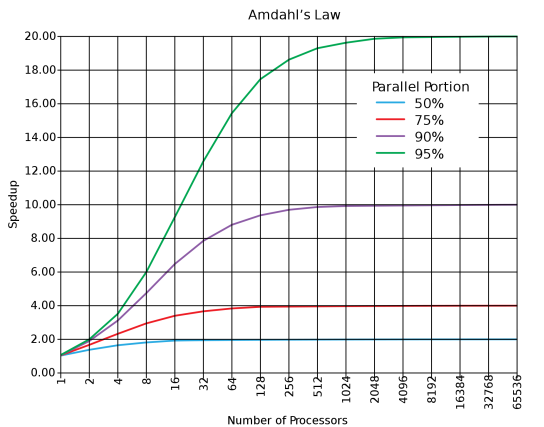
\includegraphics[width=0.3\textwidth]{amdahl}

\textbf{Amdahl's law}

$P$: proportion of programs that can be parellelized

$1-P$: proportion that remains serial

Maximum speedup that can achieved with $N$ processors: $[{(1-P) + \frac{P}{N}}]^{-1}$

\bigskip
\textbf{Kryder’s Law} Cost of storing a bit on a hard disk halves every 14 months

\bigskip
\textbf{When the neeed for parellelism arises}

\textbf{Scaling up: } A single powerful computer is added with more CPU cores, memory and
hard disks

\textbf{Scaling out: } Task is divided between a large number of less powerful machines with
relatively slow CPUs, moderate memory and moderate hard disks.

\clearpage
\textbf{mapReduce} framework that takes care of all issues related
to parallelization, synchronization, load balancing, and fault
tolerance.

\bigskip
\textbf{Hadoop Distributed File System} Open source implementation of the MapReduce framework.

\bigskip
Rack optimized. All data is replicated by default on three different data nodes (replicas) :
1.  written locally 2. Same rack 3. Another rack

\bigskip
NameNode is a single computer that maintains metadata of the file system in memory, writes
logs and does periodic snapshots to the disk

DataNodes handle block storage. Periodically sents block reports to NameNode.

\begin{minipage}{0.5\linewidth}
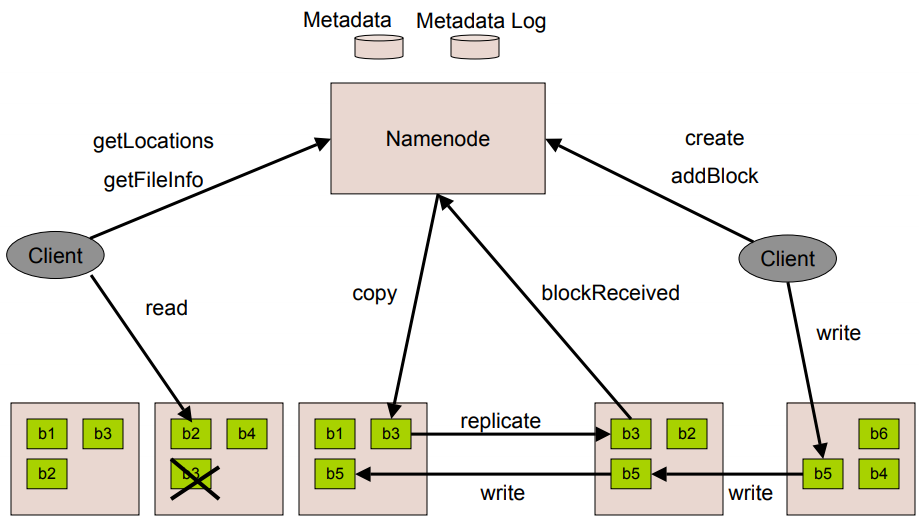
\includegraphics[width=\textwidth]{archi}
\end{minipage}
\hspace{1cm}
\begin{minipage}{0.5\linewidth}
  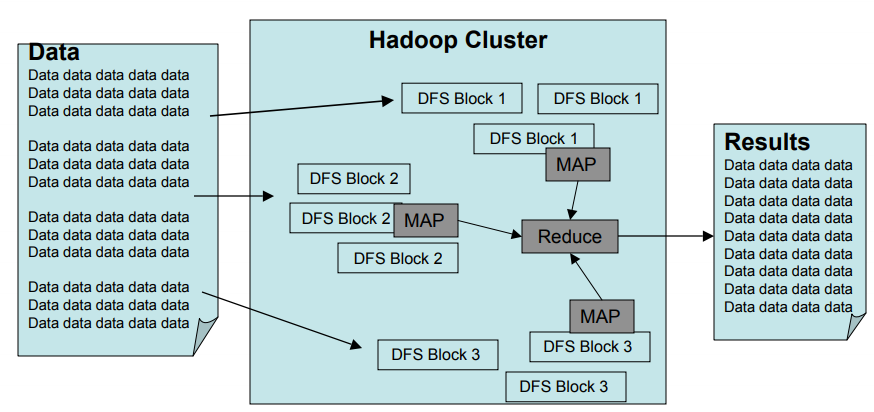
\includegraphics[width=\textwidth]{archi2}  
\end{minipage}

\bigskip
\textbf{Redundant Array of Independant Disks (RAID)} Fault tolerance mechanism

\bigskip
Raid 1: All data is stored on 2 hard disks

Raid 5: Block-level striping w. distributed parity (error protection scheme)

Raid 6: Block-level striping w. double distributed parity

Raid 10: A nested RAID level: $n$ stripes of mirrored disk pairs. Thus Data is stored on $2n$
hard disk.

\bigskip
\textbf{RAID write hole problem} A power failure during writes to a stripe can leave the Array
in a corrupted state.

\bigskip
\textbf{CAP Theorem} It's impossible to create a distributed system that satisfies all three of
the following:

\textbf{Consistent}: Every read receives the most recent write or an error

\textbf{Availability}: Every request receives a (non-error) response – without the guarantee that it contains the most recent write

\textbf{Partition Tolerance}: The system continues to operate despite an arbitrary number of messages being dropped (or delayed) by the network between nodes

\bigskip
We have to choose between 2 of the CAPs

\textbf{CA} Consistent/ Available: Non-distributed (centralized) database system

\textbf{CP} Consistent/ Partition: A distributed system that cannot be modified

\textbf{AP} Available/ Partition: A distributed system that is inconsistent

\bigskip
\textbf{Bloom Filters} highly memory efficient probabilistic data structure to store sets.
\begin{lstlisting}[language=Python]
def bloom_filter(d, k_hash_functions):
    """
    d: data item
    k_hash_functions: k independant hash functions
    Returns
        m bit vector 
    """
    B = [0 for i in range(m)]
    for h in k_hash_functions:
        hash_value = h(d)
        B[hash_value] = 1 # update
    return B          
\end{lstlisting}
\textbf{Minimizing false positives}

\textbf{Probability of false positives}

P(bit b is set to 1 by $h_i$) = $\frac{1}{m}$

P(bit b is NOT set to 1 by $h_i$) = $1 - \frac{1}{m}$

P(bit b is NOT set to 1 all k $h$) = $(1 - \frac{1}{m})^k$

P(bit b is NOT set to 1 all k $h$ after $n$ items) = $(1 - \frac{1}{m})^{kn}$

P(bit b IS set to 1 all k $h$ after $n$ items) = $(1 - \frac{1}{m})^{kn}$

P(the k bit(s) IS set to 1 all k $h$ after $n$ items) = $((1 - \frac{1}{m})^{kn})^k \approx$

p(False Positive) = $((1 - \exp(-kn/m))^{kn})^k$

\textbf{Optimal $k$} $= \frac{m}{n} \ln{(2)} \approx \frac{m}{n} \times  0.693$

\textbf{ACID/ BASE}

\clearpage
\textbf{Distributed Hash tables} uses consistent hashing to Partition a keyspace amongs
Distributed set of nodes, provide an overlay network such that the node responsible for any
can be efficiently located.

\bigskip
\textbf{Consistent Hashing} Special Hashing that when a hash table is resized, only
$\frac{K}{n}$ keys have to be remapped where $K$ is the number of keys and $n$ is the
number of array slots.

\bigskip
In distributed systems, its a way to distribute the contents of a hash table over a distributed
Hash Table (DHT). $K$ keys distributed over $n$ servers.

\bigskip
Idea:

- Key space uses 128 bits. Each computer node has a random unique node identifier
$n_i$ between $0$ to $2^{128}-1$

- All computer nodes are ordered clockwise to a virtual ring of servers with increasing node
identifier order.

- A data item with a certain key $k_j$, is stored at the node with the smallest $i$ such that
$k_j \leq n_i$. Store $k_j$ at $n_i$ where $i = min \{i : k_j \leq n_i\}$

- if a new node $k$ needs to join the virtual ring with identifier $n_k$, it will be allocated
$k_l$ for which $n_k$ is the smallest identifier such that $k_l \leq n_k$
\end{document}